\section{カルシウムイメージングデータ}
ニューロンは1ms単位で活動電位が発生する(発火).
活動電位は細胞内外のイオン濃度が局所的に変化することによって生じる.
活動電位は細胞体から軸索を伝わり,シナプスを介して結合している別のニューロンに伝わる.
哺乳類の皮質ニューロンにおいて,ニューロンからニューロンへシナプスを介して活動電位が伝わるには数十msかかる\cite{Izhikevich2004}.
このように活動電位を伝えることによってニューロン間で情報がやり取りされる.

ニューロンが他のニューロンとコネクションを持つ状態のことをコネクティビティという.
脳のコネクティビティには,synaptic connectivityとanatomical connectivityとfunctional connectivityの3種類がある.
データによってどのコネクティビティの情報を取り出せるかは異なる.

1個1個のニューロンを1ms単位で計測できればニューロン全ての活動を計測できるが,そのような技術は存在しない.
ニューロンの計測方法には様々なものがあり,それぞれ計測可能な時間分解能と空間分解能が異なる.
計測方法別の分解能については\cite{Sejnowski2014}のFig 1が分かりやすい.
EEG,PET,fMRIは脳の一部のニューロンの活動によって生じた電位,血流,代謝量の変化を計測する.
これらの手法ではニューロン単位の計測は行えないが,脳全体を計測することができる.
電気生理学的な手法やカルシウムイメージングではニューロン単位で膜電位の変化やカルシウムイオン濃度の変化を計測する.
これらの手法ではニューロン1個1個を計測できるが脳全体を計測することはできない.

カルシウムイメージングとはニューロン内のカルシウムイオン濃度を可視化することでニューロンの活動を計測する手法である.
観察したい個体のニューロンにカルシウムイオンと結合する蛍光タンパク質を発現させると,細胞内のカルシウムイオン濃度に応じて蛍光強度が変化する.
ニューロンが発火するとカルシウムイオンが流入するため蛍光強度が上昇し,その後徐々に蛍光強度は減少する.
ニューロンを蛍光顕微鏡で観察することで\Figref{fig:imaging}(B)のような蛍光強度を反映した画像が得られる.
その画像から個々のニューロンの蛍光強度のデータを取得できる.

電気生理学的な手法と比べた時のカルシウムイメージングの利点として,ニューロンの位置情報が分かるため同じニューロンを複数回観察できることとより多くのニューロンの測定ができることが挙げられる.
また,ニューロンには興奮性ニューロンと抑制性ニューロンの二種類があり,カルシウムイメージングではこの種類を見分けることができる.
二種類の蛍光タンパク質を用いて,片方の蛍光タンパク質を抑制性ニューロンのみに発現させることで興奮性・抑制性が分かる.

カルシウムイメージングが電気生理学的な手法より劣る点として,時間分解能が挙げられる.
カルシウムイメージングのサンプリングレートは測定機器に限界があり\cite{Nakamura2003},通常1Hz-50Hz程度である.
ニューロンの発火は約1msで,シナプスを介して発火が伝わるのは40ms以内\cite{Bi1998}なので,ニューロンの発火を個別に観測することはできず,低いサンプリングレートでは発火の伝達も捉えることができない.
また,カルシウムイオン濃度の変化は発火のタイムスケールより長い.
発火後に蛍光強度が変化し始めるのは数ミリ秒後,蛍光強度がピークに達するのは数100ms後である.
一方,蛍光強度が元の値に戻るまでには,数100msから数1000msかかる\cite{Hira2018}.
また,蛍光タンパク質の性能によっても時間遅れが生じる.

本研究で用いるデータは筑波大学の柳沢研究所で計測されたカルシウムイメージングデータである.
本データは,2光子多細胞カルシウムイメージングによって1匹のマウスの大脳皮質1次運動野第2・3層のニューロンのイメージング画像を得た後,人手でROIがつけられ,ニューロンごとの数値データに直されたものである.
1時間おきに15分間のイメージングが計6回行われ,各イメージングのサンプリングレートは8Hz(125msごと)である.
このサンプリングレートは使用された機器の最大のものである.
用いられた蛍光タンパク質はGCaMP6sである.
実験系は\Figref{fig:imaging}(A)の系で行われた\cite{Kanda2016}.
観測されたニューロン数は154であった.
時間方向には4sごとのマウスの状態(wake, REM, NREM)のラベルが付いており,ニューロンごとに興奮性か抑制性のラベルがついている.
\textcolor{red}{ここのデータの説明は実データ実験で使うものによって変える}

8Hzというサンプリングレートはシナプス伝達一つを見るには不十分である.
顕微鏡で観測すると活動電位が伝わる順番は分からなくなる.
そのため,カルシウムイメージングデータからはニューロンの活動の相関の情報しか得ることができないと考えられる.
また,脳の神経細胞はシナプスを3つか4つ介せば全て繋がると言われている.
これより,このデータではニューロン間のシナプス伝達を推定するのではなく,機能的に同じニューロン,つまり同時に活動するニューロングループを推定する問題が適していると考えられる.
機能的に同じニューロンは,3つの脳のコネクティビティのうちfunctional connectivityで繋がっているニューロンを指す.
\begin{figure}[htbp]
    \begin{center}
				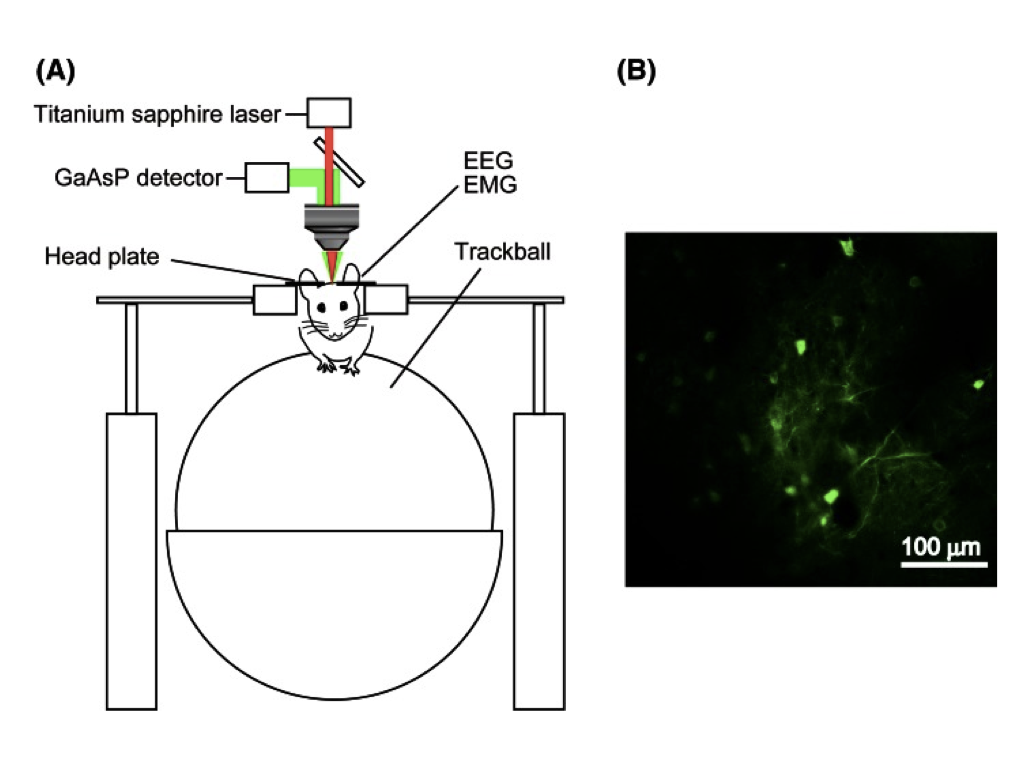
\includegraphics[width=0.8\linewidth]{imaging}
        \caption{カルシウムイメージングの測定系}
        \label{fig:imaging}
    \end{center}
\end{figure}
